\section{Results} \label{results}

\subsection{\texttt{Python} package}
Several algorithms to extract features from univariate time series had already been implemented in the \py{} package \pyeeg{}\citationneeded{}.
Unfortunately, some of them were critically slow, and could therefore not realistically have been used in the present study.
Preliminary investigation of the source code revealed that runtimes may be improved by vectorising expressions and pre-allocating of temporary arrays.
Therefore, systematic reimplementation of all algorithms in \pyeeg{} was undertaken.
Very significant improvement in performance and scalability were achieved (table~\ref{tab:benchmark}).

\begin {table}[!h]
\begin{center}
\caption{\ctit{Performance improvements over \texttt{PyEEG}.}
In order to improve performance, modifications of the algorithms implemented in \texttt{PyEEG} were carried out.
This table compares how long, on average, each algorithm would take, for a random sequence of length $1280$ (\ie{} $5s$ at $256$Hz).
It also represents how many added points would lead to a tenfold runtime increase.
For the tested range ($n \in [1280;7680] $), all algorithms add approximately an
exponential time complexity ($10^{O(n)}$, $R^2 > 0.95$, for all).
Several mathematical inconsistencies were also discovered and corrected. 
The rightmost column (\textbf{\textdagger}) indicates whether the original implementation was
corrected in order to match mathematical definition. Each alteration is mathematically justified in the section \texttt{pyrem.univariate} of the \pr{} documentation (see appendix).
\textbf{(-)}: indicates a worse performance of \pr{} over \pyeeg{}.
Significance levels: $^{***}$, $p-value < 10^{-3}$; $^{**}$, $p-value < 10^{-2}$, see Material and Methods for detail about statistical analysis.
\label{tab:benchmark}
}
\footnotesize
\begin{tabular}{|c|c|c|c|c|c|c|}
  \hline
  &  & \multicolumn{2}{|c|}{\texttt{PyEEG}} & \multicolumn{2}{|c|}{\pr} & \\
 \hline
 \hline
 
  algorithm & function & \specialcell{$t$(ms) for \\$n = 1280$} & \specialcell{$n$ for $\times 10$\\increase} & \specialcell{$t$(ms) for \\$n = 1280$} & \specialcell{$n$ for $\times 10$\\ increase} & fix\textsuperscript{\textdagger}\\
 
  \hline
  \hline
\specialcell{Approximate\\Entropy} & \texttt{ap\_ent} &                                     9970 & 4288 & $487^{***}$ & $3478^{***}(-)$ & No\\
\hline
Fisher Information & \texttt{fisher\_info} &                                 3.24 & 8673 & $0.121^{***}$ & $12427^{***}$ & No\\
\hline
\specialcell{Higuchi\\Fractal Dimension} & \texttt{hfd} &                     11.7 & 8833 & $1.39^{***}$ & $28329^{***}$ & Yes\\
\hline
Hjorth parameters & \texttt{hjorth} &                                         5.14 & 8633 & $0.088^{***}$ & $36354^{***}$ & Yes\\
\hline
\specialcell{Petrosian\\Fractal Dimension} & \texttt{pfd} &                 2.66 & 8606 & 2.65 & 8579 & Yes\\
\hline
Sample Entropy & \texttt{samp\_ent} &                                         8305 & 4276 & $188^{***}$ & $5483^{***}(-)$ & No\\
\hline
Spectral Entropy & \texttt{spectral\_entropy} &                                 0.309 & 11459 & $0.227^{***}$ & $22133^{***}$ & Yes\\
\hline
\specialcell[l]{Singular Value \\Decomposition\\ entropy} & \texttt{svd\_ent} &     3.25 & 8663 & $0.113^{***}$ & $11774^{**}$ & Yes\\
 \hline
\end{tabular}
\end{center}
\end{table}


Importantly, several mathematical inconsistancies between the original code and the mathematical definitions were also noticed.
This affected five of the eight reimplemented functions(table~\ref{tab:benchmark}). 
Detail of the corrections performed are provided, as notes, in the documentation of the new package\TODO{ref appendix}.
Numerical results for the three other functions were consitstant throughout optimisation.

In order to facilitate feature extraction, several data structures and routines were also implemented 
in a new python package named \pr{}.
Briefly, extentions of \texttt{numpy} arrays providing metadata, sampling frequency, and other attributes were used to represent time series.
User friendly indexing with string representing time was also developed.
In addition, a container for time series of discrete annotation levels, each linked to a confidence level, was built.
Importantly, a container for multiple time series, which supports different sampling frequencies
between time series was implemented.
The new package also provides visualisation, input/output, and wrappers for resampling and discrete wavelet decomposition.
Finally, unittests were implemented to ensure presistance of mathematical and programmatic validity though-out developmental stage.
A full documentation of \pr{} is provided in the appendix\TODO{ref} of the report herein.

\subsection{Variable elimination}
Including temporal features by the lag (eq.~\ref{eq:tau}) or the convolution (eq.~\ref{eq:window}) strategies, involves multiplying the number of variable, rendering computation difficult.
Therefore, variable importance was nivestigate in order to iteratively eliminate variables that did not improve predictive power.
Starting with all 164 variables, a random forests were trained, and the $1/3$ least important variables were elimitated.
This procedure was repeated iteratively and, for each iteration, the stratified cross validation error (see material and methods) was computed (fig.~\ref{fig:variable_elimination}).

\begin{figure}[h!]
  \centering    
    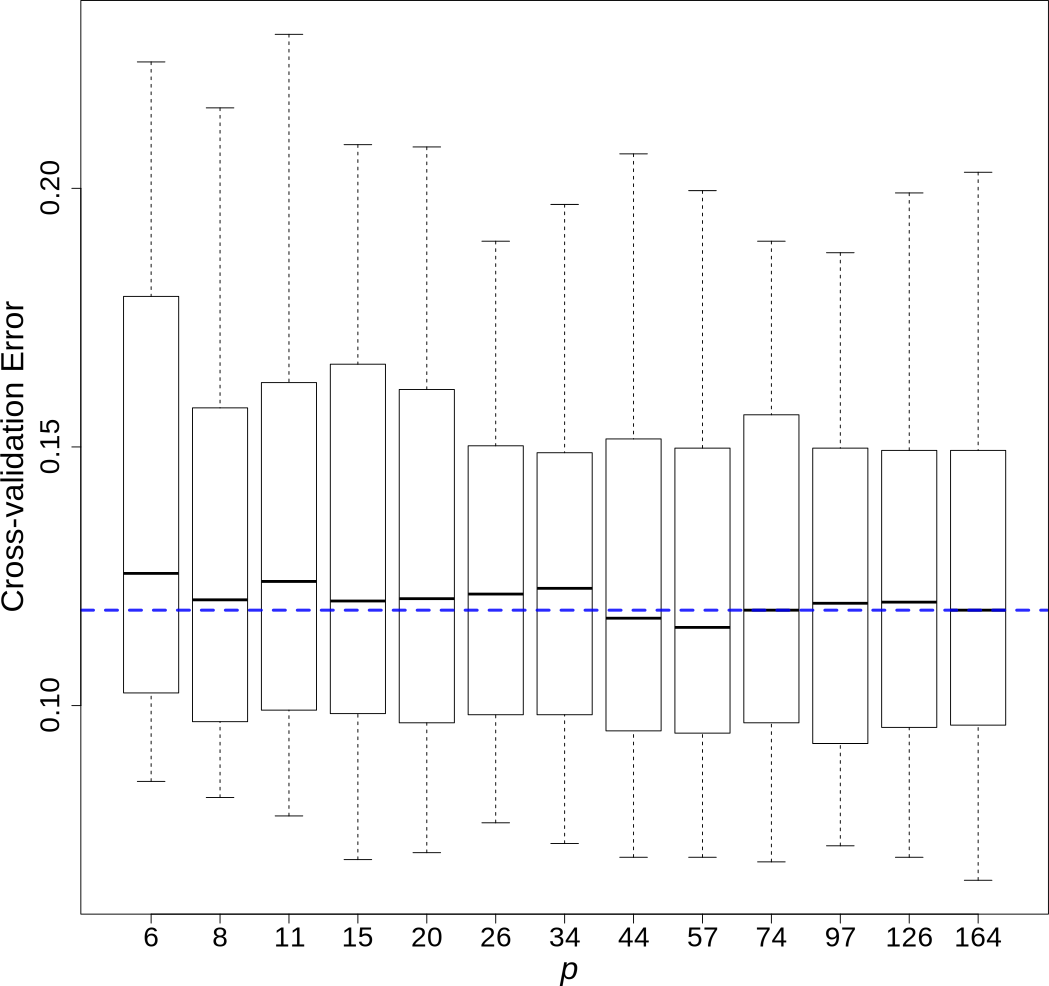
\includegraphics[width=0.5\textwidth]{figures/variable_elimination.pdf}
  \caption{\ctit{Recursive variable elimination.}
  Random forest were fitted recursively and only the most important $p/1.5$ variables were kept.
  Stratified cross-validation (see Material and Methods) was computed at each iteration. This procedure was replicated five time.
  The dashed blue line indicates the median cross-validation error when all variable are used.
  \label{fig:variable_elimination}
  }
\end{figure}


The predictive accuracy globally increases with the number of variables.
...
No stats?!
...
However, this increase is very moderate for ($p>8$) this indicates that complexity can be reduces without largely impacting accuracy.
For further investigation, $p=20$ was considered to be a good compromise between error and computationnal load.
\TODO{table importance of the 20 variables ?!}

\subsection{Including temporal information}
Manual scorer usualy use contextual information in order to make a decision conserning a given state.
For instance, implicit assumptions are made on the temporal consistency of the states (personal communications).
Therefore, it seems fair to include contextual information into an a predictor.
In this study, two different appraoches were pursued.
Either the local means of features over different ranges were added to the features of each epochs (eq.~\ref{eq:window}), 
or the features of neighbouring time points were included (eq.~\ref{eq:tau}).

A comparison of both approaches is proposed in figure \ref{fig:temporal_integration}.
Significant improvement was acchieved by both methods by including even little temporal information ($\tau = 1$, $n=\{1,3\}$).
The best accuracy was acchieved with $\tau = 2$. 
This value is also a good compromise because it only inflates $p$ by five fold.
In addition, it is advantageaout to requiere only the two previous and next values as oposed to have to integrates minutes of information around the epoch of interest.

\begin{figure}[h!]
  \centering    
    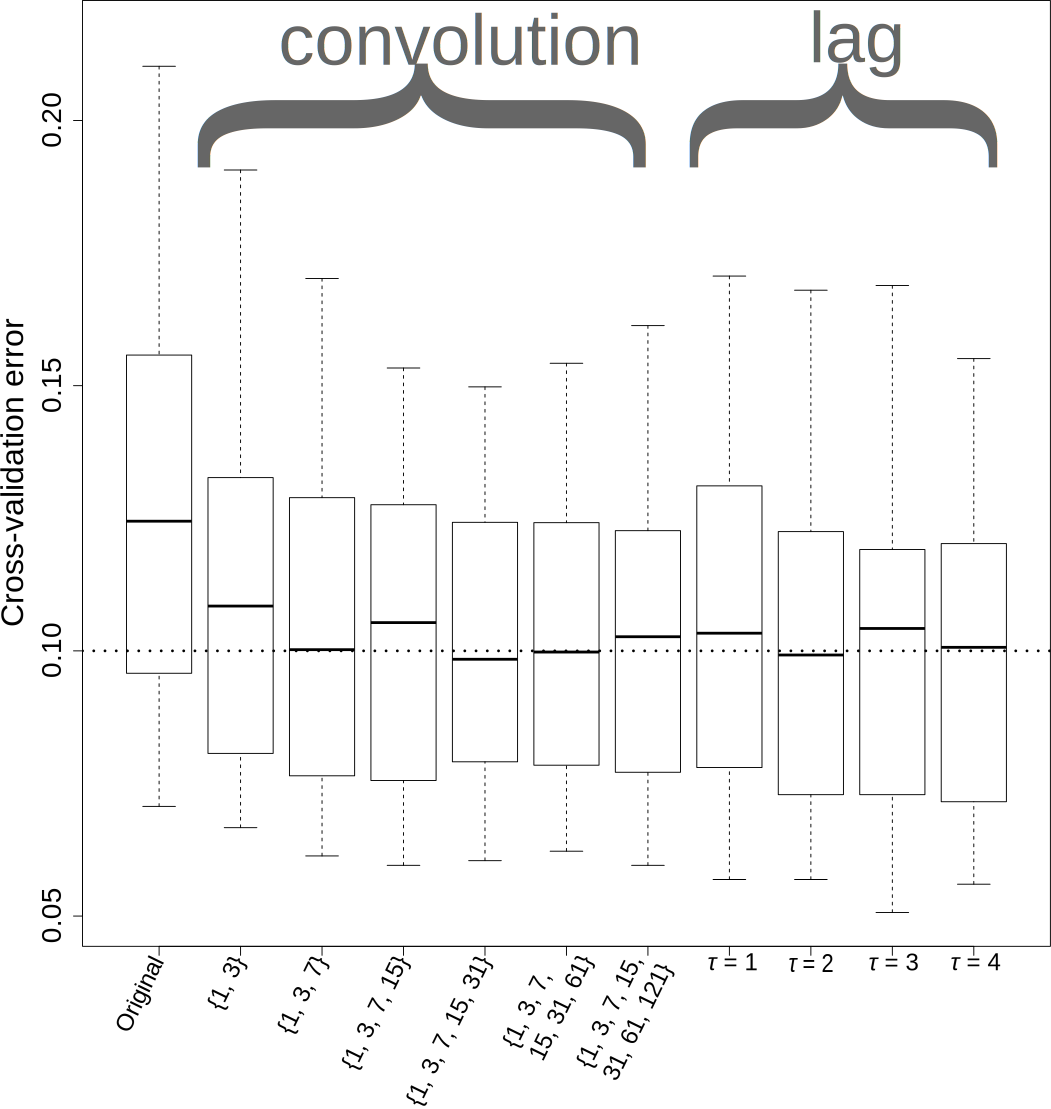
\includegraphics[width=0.5\textwidth]{figures/temporal_integration.pdf}
  \caption{\ctit{Integration of temporal information.}
  In order to improve prediction accuracy, information about the past and future features was added to the original features following two different strategies.
  Convolution inflates $p$ by adding the mean features of neighbouring points over different window sizes (eq.~\ref{eq:window}).
  The numbers in braces represent the window sizes.
  Alternatively, the features of the $\tau$ previous and future neighbours was added to the variables (eq.~\ref{eq:tau}).
  The dotted line represents a cross-validation error of $10\%$.
  All additions of temporal features reduce significantly the cross-validation error compared to the original set of features ($p-value < 5.10^{-3}$, for all, repeated t-tests).
  Significance threshold, $\alpha = 0.05$, after Bonferroni correction is $\alpha' = 0.05/10 = 5.10^{-3}$.
  \label{fig:temporal_integration}
  }
\end{figure}

Combining both approches did not improve the predictor any further (data not shown).

\subsection{Prediction results}

In order to study the relationship between $c$ and the probability of error,
the average cross-validation error was computed for different degrees of confidence (fig\ref{fig:error}A).
As expected, the probability of misclassification decreases monotonicaly with $c$.

As oposed to previous results, the final random forests were trained, and tested, with sub-samples accounting for the respective biological prevalence of the three stages (\ie{} unbalanced).
Only the top N\TODO{} important variables \TODO{ref table}, were used. Temporal information was included using eq.\ref{eq:tau}\TODO{ref}.



